\documentclass[a4paper,10pt]{report}

\usepackage[utf8]{inputenc}
\usepackage{amsmath, amssymb, hyperref, multirow, dot2texi}

\usepackage{tikz}
\usetikzlibrary{shapes, arrows}

% Title Page
\title{}
\author{}

\begin{document}

Collapsed Segmented LDA (CSLDA):

$$ p(S, Z, W | \alpha, \beta, \eta, \sigma) = \left[ \prod_k \frac{\Gamma(W \beta)}{\Gamma(\beta)^W \cdot \Gamma(N_k + W \beta)} \prod_w \Gamma(N_{kw} + \beta) \right] $$
$$ \times \left[ \prod_d \mathcal{N}\left(s_d\, \left|\, \eta^T \cdot \frac{N_{dk}}{N_d}, \sigma\right. \right) \frac{\Gamma(K \alpha)}{\Gamma(\alpha)^K \cdot \Gamma(N_d + K \alpha)} \prod_k \Gamma(N_{dk} + \alpha) \right] $$

Where we used $ \frac{N_{dk}}{N_d} \equiv \bar{Z_d} $

$$ \log p(S, Z, W | \alpha, \beta, \eta, \sigma) = $$
$$ \left[ \sum_k \log \Gamma(W \beta) - W \log \Gamma(\beta) - \log \Gamma(N_k + W \beta) + \sum_w \log \Gamma(N_{kw} + \beta) \right] $$
$$ + \left[ \sum_d \underbrace{- \log \sigma - \frac{1}{2} \log(2 \pi) - \frac{\left(s_d - \eta^T \cdot \frac{N_{dk}}{N_d}\right)^2}{2 \sigma^2}}_{\text{Normal distribution}} + \right. $$
$$ \left. \log \Gamma(K \alpha) - K \log \Gamma(\alpha) - \log \Gamma(N_d + K \alpha) + \sum_k \log \Gamma(N_{dk} + \alpha) \right] $$

Maximum a posteriori (MAP) estimate for the $\eta$ hyperparameter:

$$ \nabla_{\eta_k} \log p(S, Z, W | \alpha, \beta, \eta, \sigma) = \sum_d \frac{ \frac{N_{dk}}{N_d} \left( s_d - \eta^T \frac{N_{d\cdot}}{N_d}\right) }{\sigma^2} = $$
$$ = \sum_d \frac{s_d \frac{N_{dk}}{N_d} }{\sigma^2} - \sum_d \frac{ \frac{N_{dk}}{N_d} \left( \eta^T \frac{N_{d\cdot}}{N_d} \right) }{\sigma^2} = 0 $$
$$ \Rightarrow \sum_d s_d \frac{N_{dk}}{N_d} = \sum_d \frac{N_{dk}}{N_d} \left( \sum_{k'} \eta_{k'} \frac{N_{dk'}}{N_d} \right) = \sum_d \frac{N_{dk}}{N_d} \left( \eta_k \frac{N_{dk}}{N_d} + \sum_{k' \ne k} \eta_{k'} \frac{N_{dk'}}{N_d} \right) $$
$$ \Rightarrow \sum_d s_d \frac{N_{dk}}{N_d} = \eta_k \sum_d \left( \frac{N_{dk}}{N_d}  \right)^2 + \sum_d \left( \frac{N_{dk}}{N_d} \sum_{k' \ne k} \eta_{k'} \frac{N_{dk'}}{N_d} \right) $$
$$ \Rightarrow \sum_d \left( s_d \frac{N_{dk}}{N_d} - \frac{N_{dk}}{N_d} \sum_{k' \ne k} \eta_{k'} \frac{N_{dk'}}{N_d} \right) = \eta_k \sum_d \left( \frac{N_{dk}}{N_d}  \right)^2 $$
$$ \Rightarrow \sum_d \frac{N_{dk}}{N_d} \left( s_d - \sum_{k' \ne k} \eta_{k'} \frac{N_{dk'}}{N_d} \right) = \eta_k \sum_d \left( \frac{N_{dk}}{N_d}  \right)^2 $$
$$ \Rightarrow \eta_k = \frac{\sum_d \frac{N_{dk}}{N_d} \left( s_d - \sum_{k' \ne k} \eta_{k'} \frac{N_{dk'}}{N_d} \right)}{\sum_d \left( \frac{N_{dk}}{N_d}  \right)^2} $$

Trying to apply the previous formula as an update rule for $\eta$ does not converge. Instead, the following update can be used:

\begin{multline*}
\eta_k^{new} \leftarrow (1 - \gamma) \eta_k^{old} + \gamma \frac{\sum_d \frac{N_{dk}}{N_d} \left( s_d - \sum_{k' \ne k} \eta_{k'}^{old} \frac{N_{dk'}}{N_d} \right)}{\sum_d \left( \frac{N_{dk}}{N_d}  \right)^2 + \varepsilon}
\end{multline*}

With $1 \gg \gamma > 0$ in order for the previous series to converge and $1 \gg \epsilon > 0$ is a smoothing constant.

Gibbs sampler:

\begin{multline*}
p(z_{di} = k \mid Z^{\backslash i}, S, W, \alpha, \beta, \eta, \sigma) \propto p(z_{di} = k, Z_{-i}, S, W, \alpha, \beta, \eta, \sigma) \\
\propto \left[ \prod_{k'} \frac{\prod_w \Gamma(N_{{k'}w}^{\backslash i} + \mathbb{I}(k' = k \wedge w = w_{di}) + \beta)}{\Gamma(N_{k'}^{\backslash i} + \mathbb{I}(k' = k) + W \beta)} \right] \times \\
\underbrace{\mathcal{N}\left(s_d\, \left|\, \eta^T \cdot \frac{N_{d{k'}}^{\backslash i} + \mathbb{I}(k' = k)}{N_d}, \sigma\right. \right)}_\text{Movie score term} \prod_{k'} \Gamma(N_{d{k'}}^{\backslash i} + \mathbb{I}(k' = k) + \alpha)
\end{multline*}

\begin{multline*}
\log \left[ \prod_{k'} \frac{\prod_w \Gamma(N_{{k'}w}^{\backslash i} + \mathbb{I}(k' = k \wedge w = w_{di}) + \beta)}{\Gamma(N_{k'}^{\backslash i} + \mathbb{I}(k' = k) + W \beta)} \right] = \\
\sum_{k'} \left[ \sum_w \log \Gamma(N_{{k'}w}^{\backslash i} + \mathbb{I}(k' = k \wedge w = w_{di}) + \beta) \right] - \log \Gamma(N_{k'}^{\backslash i} + \mathbb{I}(k' = k) + W \beta) = \\
\sum_{k'} \sum_w \log \Gamma(N_{{k'}w}^{\backslash i} + \mathbb{I}(k' = k \wedge w = w_{di}) + \beta) - \sum_{k'} \log \Gamma(N_{k'}^{\backslash i} + \mathbb{I}(k' = k) + W \beta) = \\
\sum_w \sum_{k'} \sum_{j = 0}^\infty \log \left(N_{{k'}w}^{\backslash i} + \mathbb{I}(k' = k \wedge w = w_{di}\right) + \beta + j) + \log \left(N_{k'}^{\backslash i} + \mathbb{I}(k' = k) + W \beta + j\right)
\end{multline*}

\begin{multline*}
 \log \left( \prod_{k'} \Gamma(N_{d{k'}}^{\backslash i} + \mathbb{I}(k' = k) + \alpha) \right) \propto \\
- \sum_{k'} \sum_{j = 0}^\infty \log (N_{dk'}^{\backslash i} + \mathbb{I}(k' = k) + \alpha + j)
\end{multline*}
 
\subsection*{Dataset}

\begin{itemize}
	\item Number of movies $\approx$ 700
	\item Distribution of movie scores:
	
	\begin{figure}[ht!]
		\centering
		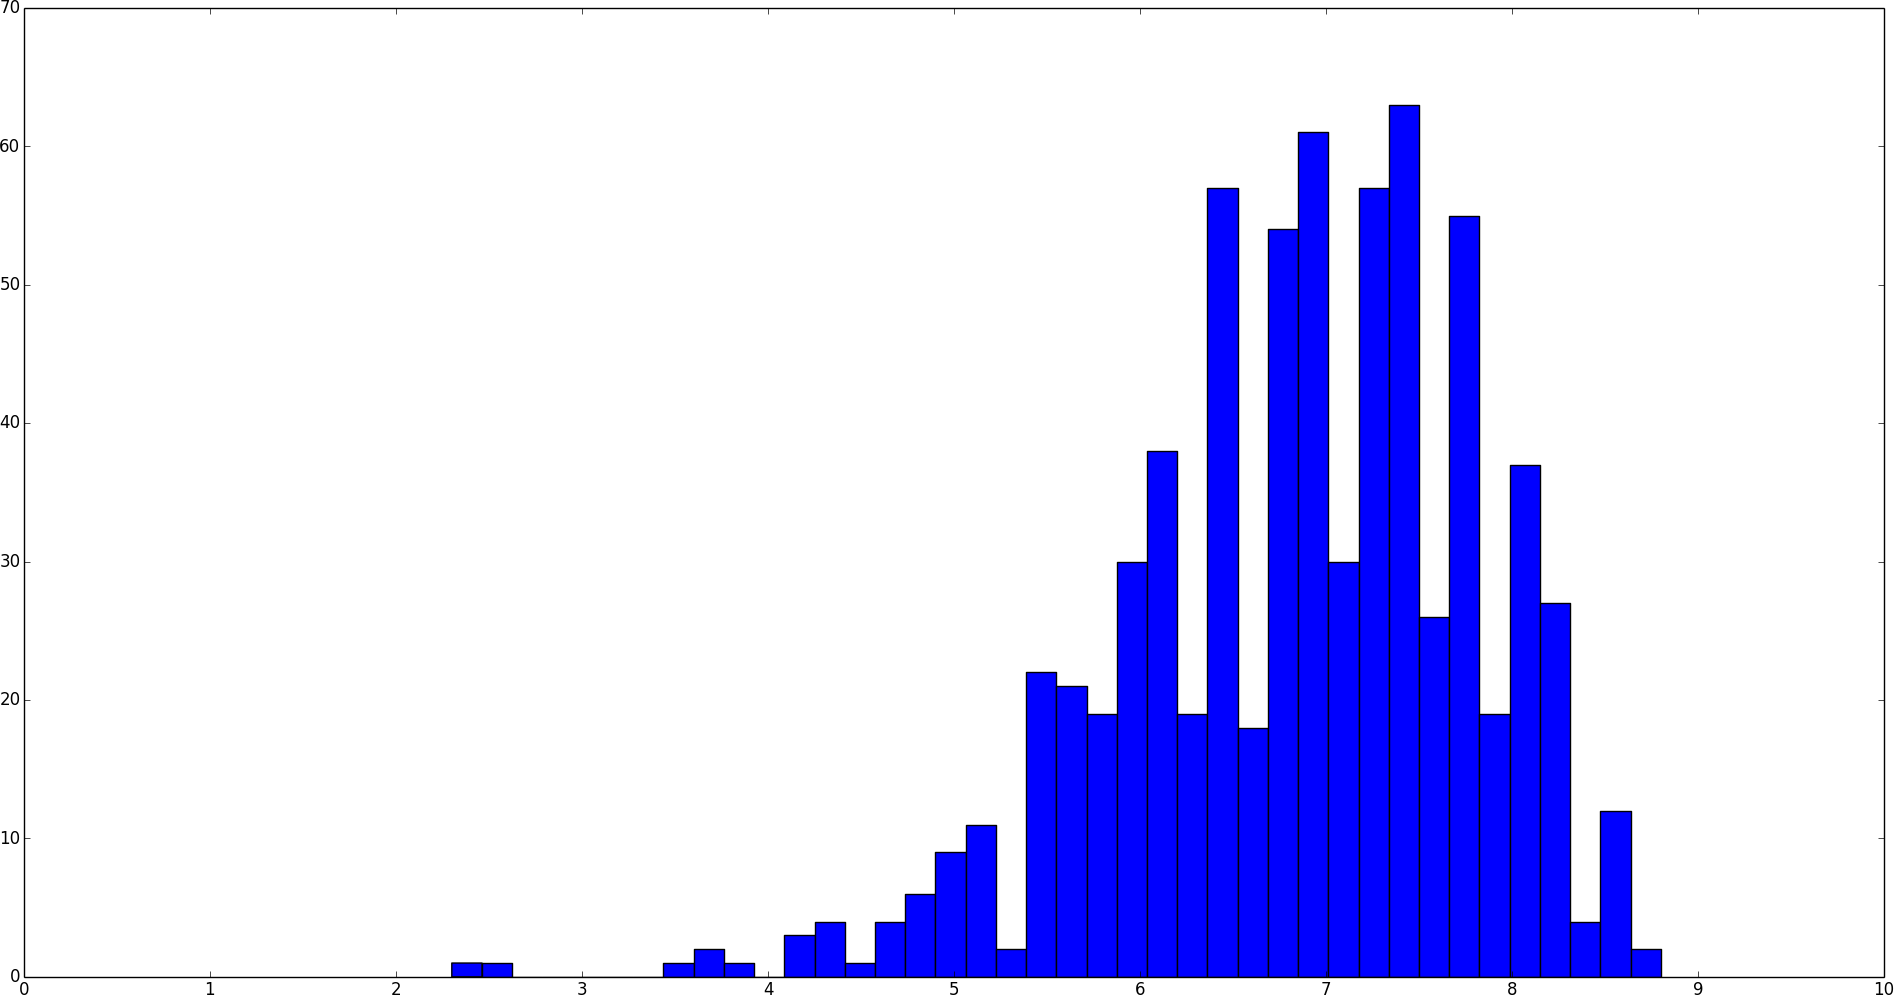
\includegraphics[width=\textwidth]{scores_histogram.png}
		
		\caption{Moo}
	\end{figure}

	\item Average number of tokens within a movie summary $\approx$ 75
	\item Average number of tokens within a movie script $\approx$ 18000
	\item Most frequent tokens (stemmed words):
	
	\begin{figure}[ht!]
		\centering
		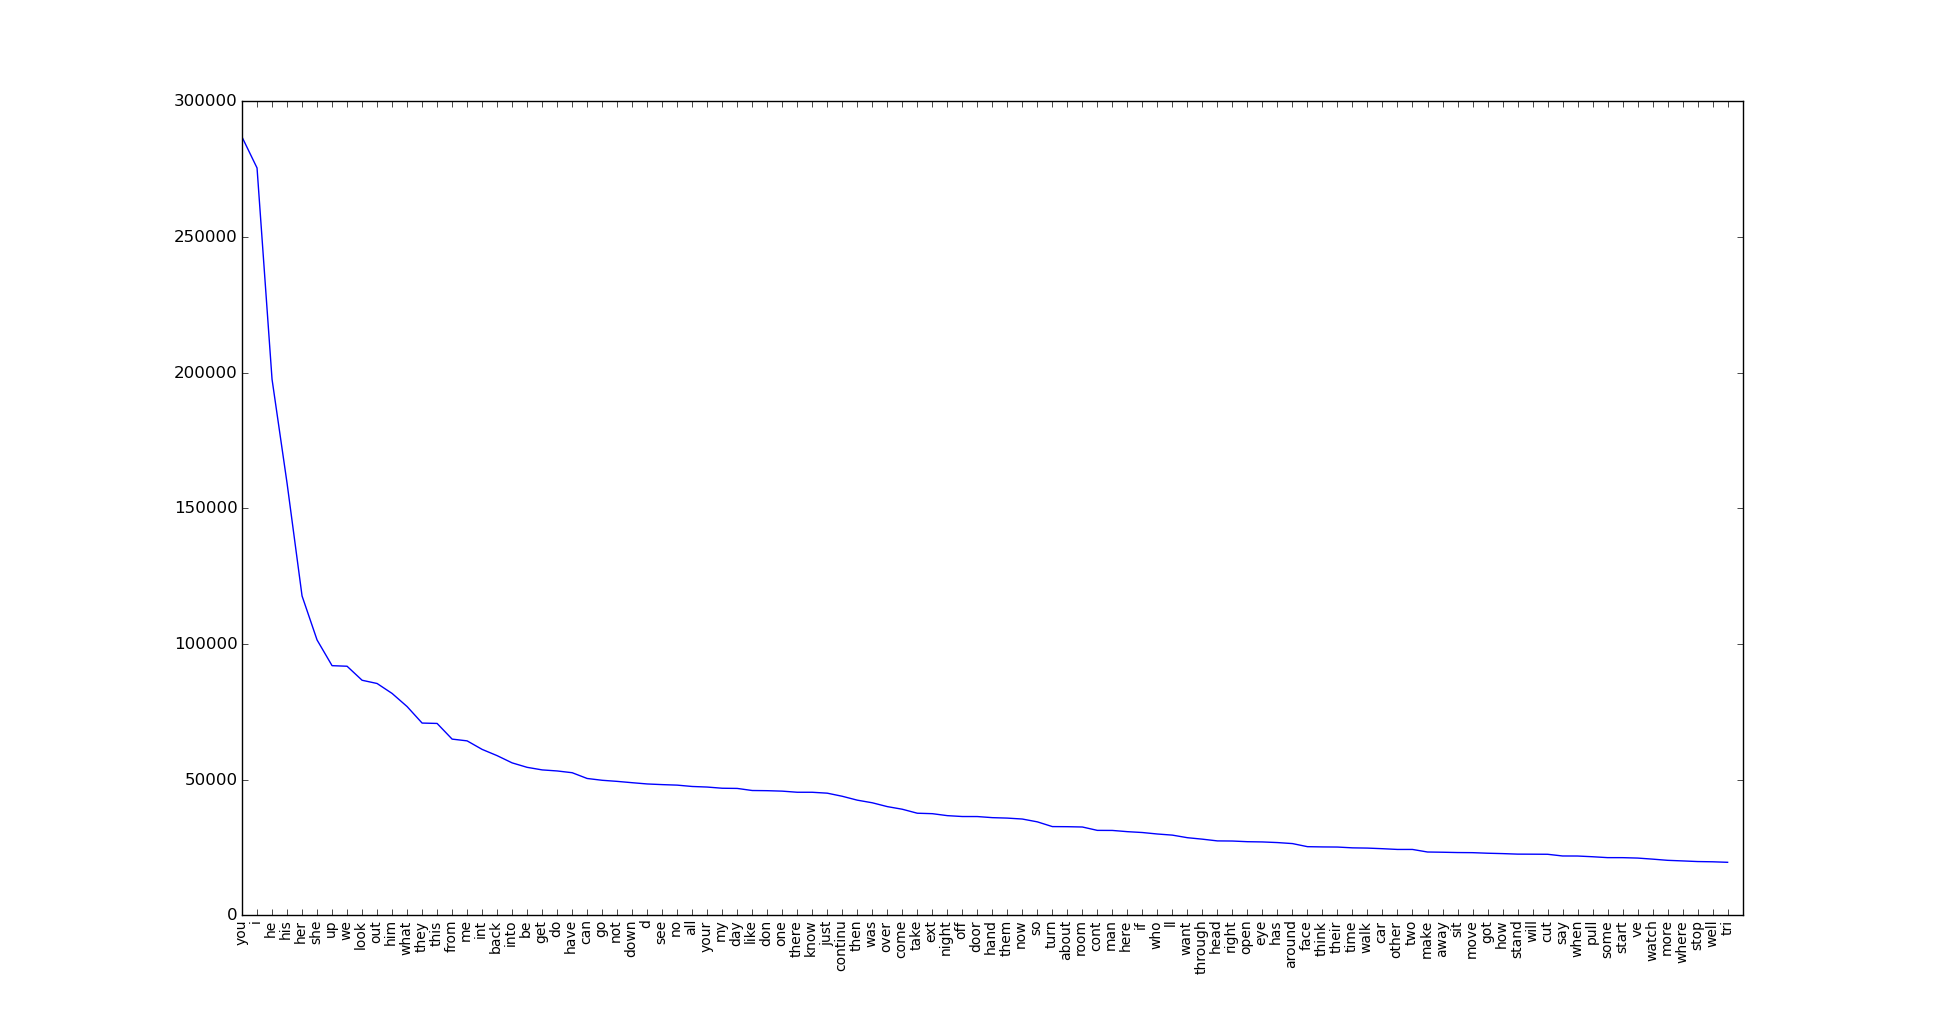
\includegraphics[width=\textwidth]{most_frequent_tokens_global.png}
		
		\caption{Most frequent tokens}
	\end{figure}
\end{itemize}


Results with 5 movies in the training set and 5 movies in the testing set (5 burn-in, 3 skip, 5 samples):

Perplexity values:

% For K = 5:
% Model perplexity       = 9839.41
% Model inverse accuracy = 952.49
% Model perplexity       = 9727.80
% Model inverse accuracy = 954.52

% For K = 10:
% Model perplexity       = 9068.27
% Model inverse accuracy = 920.19

\begin{center}
	\begin{tabular}{cc|ccc}
	K &  & 5 & 10 & 20 \\ \hline
	\multirow{2}{*}{Using scores?} & Yes & 10059 & 7503 & 10938   \\
	& No  & 9297 & 10180 & 9663   \\
	\end{tabular}
\end{center}

Inverse accuracy values:

\begin{center}
	\begin{tabular}{cc|ccc}
	K &  & 5 & 10 & 20 \\ \hline
	\multirow{2}{*}{Using scores?} & Yes & 964 & 703 & 1133   \\
	& No  & 915 & 1143 & 960   \\
	\end{tabular}
\end{center}

\end{document}          
